
%(BEGIN_QUESTION)
% Copyright 2014, Tony R. Kuphaldt, released under the Creative Commons Attribution License (v 1.0)
% This means you may do almost anything with this work of mine, so long as you give me proper credit

Predict the long-term effects of the steam temperature increasing.  Assume all loop components are properly configured, that the controller is well-tuned, and that a significant amount of time has passed since the temperature of the steam supplied by the boiler has increased.  Compare these conditions with what they were before the process change:

$$\includegraphics[width=15.5cm]{i03335x01.eps}$$

\begin{itemize}
\item{} Steam valve will: {\it open up} further, {\it close down} more, or {\it remain in the same position} 
\vskip 10pt
\item{} Product temperature will: {\it increase} from what it was before, {\it decrease} from what it was before, or {\it remain the same} as before
\end{itemize}

\underbar{file i03335}
%(END_QUESTION)





%(BEGIN_ANSWER)

\begin{itemize}
\item{} Steam valve will: {\bf close down} more 
\vskip 5pt
\item{} Product temperature will: {\bf remain the same}
\end{itemize}

%(END_ANSWER)





%(BEGIN_NOTES)

{\bf This question is intended for exams only and not worksheets!}.

%(END_NOTES)



